\documentclass[12pt,a4paper]{article}

\usepackage{geometry}
\geometry{margin=1in}

\usepackage{graphicx}
\usepackage{float}
\usepackage{amsmath}
\usepackage{booktabs}
\usepackage{tikz}
\usepackage{pgfplots}
\pgfplotsset{compat=1.18}

\usepackage{hyperref}

\title{\textbf{Lab 1: Message Passing Interface (MPI)}}
\author{Ahmad Bin Rashid}
\date{}

\begin{document}

\begin{titlepage}

\title{
    \vspace{1cm}
    \textbf{\Huge Lab 1 Report} \\
    \vspace{0.5cm}
    \large Message Passing Interface (MPI) \\
    \vspace{2.5cm}
}

\author
{\Large \textbf{Name:} Ahmad Bin Rashid \\ [0.5cm]\\
\Large \textbf{Roll No:} 2023-CS-53 \\ [0.5cm]\\
\Large \textbf{Instructor:} Sir Waqas Ali \\ [0.5cm]\\
\Large \textbf{Course:} Distributed and Parallel Computing \\ [0.5cm]\\ 
\Large \textbf{University of Engineering and Technology} \\ [0.5cm]\\ }

\begin{figure}
    \centering
    \vspace{1cm}
    \includegraphics[width=0.3\textwidth]{uet-lahore-seeklogo.png}
\end{figure}

\date{\today}

\end{titlepage}

% --- Title Page ---
\maketitle
\thispagestyle{empty}
\newpage

\section{Introduction}
The objective of this lab is to understand distributed-memory parallel
programming using the Message Passing Interface (MPI).
The lab explores process-based parallelism, inter-process communication,
and performance scalability using multiple MPI programs.

%-------------------------------------------------
\section{Tools and Environment}

\begin{itemize}
  \item Programming Language: C
  \item Parallel Framework: MPI (OpenMPI)
  \item Compiler: \texttt{mpicc}
  \item Execution Tool: \texttt{mpirun}
  \item Operating System: Linux
\end{itemize}

%-------------------------------------------------
\section{Programs Implemented}

\begin{itemize}
  \item Hello World using MPI
  \item Ping-Pong Communication Benchmark
  \item Parallel Counting using MPI
  \item Parallel Computation of $\pi$ using MPI
\end{itemize}

%-------------------------------------------------
\section{Hello World (MPI)}

Each MPI process prints its rank and the total number of processes.
This program demonstrates basic MPI initialization, rank identification,
and parallel execution.

\begin{figure}[H]
\centering
\includegraphics[width=0.9\textwidth]{hello-mpi.png}
\caption{MPI Hello World Execution}
\end{figure}

%-------------------------------------------------
\section{Ping-Pong Communication}

The ping-pong program measures message latency between two MPI processes
by repeatedly sending and receiving messages.

\textbf{Observed Results:}
\begin{itemize}
  \item Total Time: 0.846861 seconds
  \item Average Round-Trip Time: 84.686075 microseconds
\end{itemize}

\begin{figure}[H]
\centering
\includegraphics[width=0.9\textwidth]{pingpong.png}
\caption{Ping-Pong Communication Results}
\end{figure}

%-------------------------------------------------
\section{Parallel Counting using MPI}

The workload is divided among MPI processes, and each process computes a
partial count. The final result is obtained using reduction.

\subsection{Execution Screenshots}
\begin{figure}[H]
\centering
\includegraphics[width=0.9\textwidth]{count-mpi-1.png}
\caption{Count Program Execution Results}
\end{figure}
\begin{figure}[H]
\centering
\includegraphics[width=0.9\textwidth]{count-mpi2.png}
\caption{Count Program Execution Results}
\end{figure}


\subsection{Execution Time}

\begin{table}[H]
\centering
\begin{tabular}{c c}
\toprule
\textbf{Processes} & \textbf{Execution Time (s)} \\
\midrule
1 & 0.326666 \\
2 & 0.130052 \\
3 & 0.107822 \\
4 & 0.092276 \\
5 & 0.082485 \\
6 & 0.074176 \\
8 & 0.095561 \\
\bottomrule
\end{tabular}
\caption{MPI Counting Execution Time}
\end{table}

\subsection{Speedup Graph}

\begin{figure}[H]
\centering
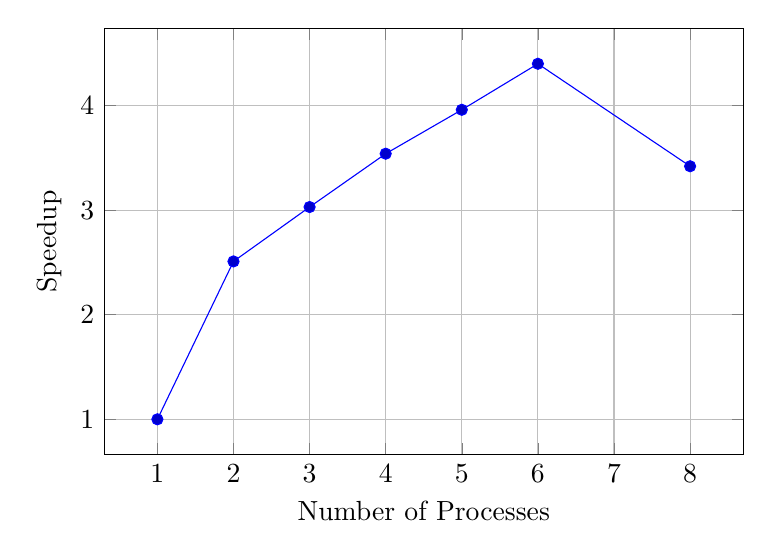
\begin{tikzpicture}
\begin{axis}[
    xlabel={Number of Processes},
    ylabel={Speedup},
    grid=major,
    width=0.8\textwidth,
    height=7cm
]
\addplot coordinates {
(1,1.00)
(2,2.51)
(3,3.03)
(4,3.54)
(5,3.96)
(6,4.40)
(8,3.42)
};
\end{axis}
\end{tikzpicture}
\caption{Speedup for MPI Counting Program}
\end{figure}

%-------------------------------------------------
\section{Parallel Computation of $\pi$}

The value of $\pi$ is approximated using numerical integration.
The computation is distributed across MPI processes.

\subsection{Execution Screenshots}
\begin{figure}[H]
\centering
\includegraphics[width=0.9\textwidth]{pi-mpi-1.png}
\caption{Pi Program Execution Results}
\end{figure}
\begin{figure}[H]
\centering
\includegraphics[width=0.9\textwidth]{pi-mpi-2.png}
\caption{Pi Program Execution Results}
\end{figure}

\subsection{Execution Time}

\begin{table}[H]
\centering
\begin{tabular}{c c}
\toprule
\textbf{Processes} & \textbf{Execution Time (s)} \\
\midrule
1 & 5.675158 \\
2 & 2.731667 \\
3 & 2.547047 \\
4 & 2.072882 \\
5 & 2.008539 \\
6 & 1.850164 \\
8 & 1.715379 \\
10 & 2.583654 \\
\bottomrule
\end{tabular}
\caption{MPI $\pi$ Computation Execution Time}
\end{table}

\subsection{Speedup Graph}

\begin{figure}[H]
\centering
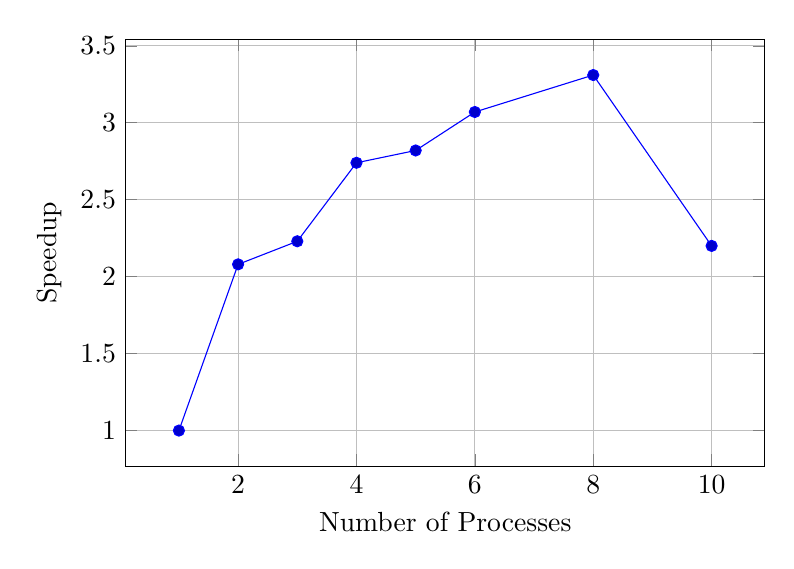
\begin{tikzpicture}
\begin{axis}[
    xlabel={Number of Processes},
    ylabel={Speedup},
    grid=major,
    width=0.8\textwidth,
    height=7cm
]
\addplot coordinates {
(1,1.00)
(2,2.08)
(3,2.23)
(4,2.74)
(5,2.82)
(6,3.07)
(8,3.31)
(10,2.20)
};
\end{axis}
\end{tikzpicture}
\caption{Speedup for MPI $\pi$ Computation}
\end{figure}

\section{Comparison: Pthreads vs MPI Counting Program}

This section compares the Pthreads and MPI implementations of the counting
program based on their measured execution times on the same machine.

\subsection{Execution Time Comparison}

\begin{table}[H]
\centering
\begin{tabular}{c c c}
\toprule
\textbf{Workers} & \textbf{Pthreads Time (s)} & \textbf{MPI Time (s)} \\
\midrule
1 & 0.13 & 0.326666 \\
2 & 0.13 & 0.130052 \\
3 & --   & 0.107822 \\
4 & 0.58 & 0.092276 \\
5 & --   & 0.082485 \\
6 & 0.25 & 0.074176 \\
8 & 0.24 & 0.095561 \\
\bottomrule
\end{tabular}
\caption{Execution Time Comparison of Pthreads and MPI Counting Programs}
\end{table}

\subsection{Discussion}

For a single worker, the Pthreads version performs significantly faster than
the MPI version due to lower overhead and direct access to shared memory.
As the number of workers increases, the MPI implementation shows better
scalability and consistently lower execution times, especially from 3 to
6 processes.

The Pthreads implementation exhibits irregular performance, particularly at
4 threads, where contention and synchronization overhead dominate.
MPI avoids shared-memory contention by using independent processes, resulting
in more stable scaling.

At higher worker counts, oversubscription causes MPI performance to degrade,
as seen at 8 processes.
Overall, Pthreads are more efficient for small-scale shared-memory parallelism,
while MPI provides better scalability and predictability for larger parallel
configurations.

\section{Self-Assessment Questions}

\begin{enumerate}

\item \textbf{What are the main limitations of shared-memory parallelism that motivate the use of distributed memory?} \\
Shared-memory systems are limited by memory bandwidth, cache coherence
overhead, and contention for shared resources.
They also scale poorly beyond a single machine.
Distributed-memory systems avoid these bottlenecks by using private memory
per process and explicit communication.

\item \textbf{Explain the SPMD model and how it is used in MPI.} \\
SPMD stands for \emph{Single Program, Multiple Data}.
In MPI, all processes execute the same program but operate on different
portions of the data.
Each process behaves differently based on its rank, enabling parallel
execution without separate programs.

\item \textbf{Why does each MPI process generate its own random data in the counting program? What are the trade-offs?} \\
Having each process generate its own data avoids the overhead of distributing
large arrays from a single process.
This improves scalability and reduces communication cost.
However, it may increase total memory usage and reduce reproducibility.

\item \textbf{What would happen if \texttt{MPI\_Bcast} for \texttt{n} were omitted in the $\pi$ program?} \\
Without \texttt{MPI\_Bcast}, different processes may use uninitialized or
inconsistent values of \texttt{n}.
This would lead to incorrect or undefined results.
The broadcast ensures all processes perform the same amount of computation.

\item \textbf{Why is MPI\_Send/MPI\_Recv much slower than updating a shared variable in Pthreads?} \\
MPI communication involves data copying, buffering, and protocol overhead.
In contrast, updating a shared variable in Pthreads is a simple memory
operation protected by a lock.
The difference arises due to inter-process communication versus shared memory.

\item \textbf{What do you observe when running ping-pong with different message sizes?} \\
For small messages, latency dominates and round-trip time increases slowly.
As message size grows, bandwidth becomes the limiting factor and time
increases linearly.
This shows the transition from latency-bound to bandwidth-bound communication.

\item \textbf{According to Amdahl’s Law, what is the maximum speedup with 95\% parallelism on 8 processors?} \\
The theoretical speedup is approximately $1 / (0.05 + 0.95/8) \approx 5.93$.
The measured speedup is lower due to communication overhead and load imbalance.
This discrepancy highlights practical limits of parallel execution.

\item \textbf{Why might MPI show lower efficiency than Pthreads on a single machine?} \\
MPI incurs overhead from message passing, data copying, and process management.
Pthreads use shared memory and lightweight synchronization.
On a single node, MPI communication costs are higher than thread-based access.

\item \textbf{Compare MPI\_Scatter with local data generation in the counting program.} \\
Using \texttt{MPI\_Scatter} centralizes data generation but increases
communication overhead.
Local data generation improves scalability and reduces memory traffic.
However, scattering provides better control over data consistency.

\item \textbf{Which programming model would you use on a 100-node cluster and why?} \\
MPI is required to scale across multiple nodes in a cluster.
Pthreads can be combined with MPI using a hybrid model where MPI handles
inter-node communication and Pthreads exploit intra-node parallelism.
This approach maximizes performance and resource utilization.

\end{enumerate}

\section{Reflection}

Moving from shared-memory programming using Pthreads to distributed-memory
programming using MPI was both challenging and insightful.
In shared-memory systems, communication is implicit, which makes programming
simpler but introduces risks such as race conditions and deadlocks.
MPI requires explicit communication, which initially feels more complex but
results in cleaner data ownership and better isolation.

The most surprising aspect of MPI was how eliminating shared memory removed
the need for locks and mutexes entirely.
Instead, correctness depends on proper message ordering and collective
operations.
The most difficult part was understanding how to divide work evenly among
processes and correctly combine partial results.

Debugging MPI programs was also more challenging due to multiple processes
running independently.
However, MPI programs scaled better and behaved more predictably under load.
Overall, this lab improved my understanding of distributed systems and showed
why MPI is widely used in high-performance computing environments.

%-------------------------------------------------
\section{Analysis and Discussion}

Speedup improves with an increasing number of processes, but does not scale
linearly due to communication overhead, synchronization costs, and limited
hardware resources. Oversubscription results in diminishing returns and
performance degradation beyond a certain point.

The $\pi$ computation shows better scalability than the counting program
because it has a higher computation-to-communication ratio.

%-------------------------------------------------
\section{Conclusion}

This lab demonstrated the fundamentals of distributed-memory parallel
programming using MPI. MPI allows true parallel execution across processes
and scales better than threading for CPU-bound workloads. However, efficient
parallelization requires careful consideration of communication overhead
and process placement.


\end{document}